\documentclass[a4paper,12pt]{article}
\usepackage{times}
\usepackage[english]{babel}
\usepackage{natbib}
\usepackage{url}
\usepackage[utf8x]{inputenc}
%\usepackage{amsmath}
\usepackage{graphicx}
\graphicspath{{images/}}
\usepackage{parskip}
\usepackage{fancyhdr}
\usepackage{vmargin}
\usepackage{setspace}
\setmarginsrb{3 cm}{2.5 cm}{3 cm}{2.5 cm}{1 cm}{1.5 cm}{1 cm}{1.5 cm}

\title{Assignment 1 - Project Phase 1}								% Title
\author{Giovanni Mostert}								      % Author
\date{\today}											      % Date

\makeatletter
\let\thetitle\@title
\let\theauthor\@author
\let\thedate\@date
\makeatother

\pagestyle{fancy}
\fancyhf{}
\rhead{\theauthor}
\lhead{\thetitle}
\cfoot{\thepage}
\spacing{1.213}

\begin{document}

%%%%%%%%%%%%%%%%%%%%%%%%%%%%%%%%%%%%%%%%%%%%%%%%%%%%%%%%%%%%%%%%%%%%%%%%%%%%%%%%%%%%%%%%%

\begin{titlepage}
	\centering
    \vspace*{0.5 cm}
    
\includegraphics[scale = 0.75]{NUST.png}\\[0.5 cm]	            % University Logo
    \textsc{\LARGE Namibia University}\\[0.4 cm]
    \textsc{\LARGE of Science and Technology}\\[2.0 cm]	            % University Name
	\textsc{\Large MMA710S}\\[0.5 cm]				      % Course Code
	\textsc{\large Multimedia Applications}\\[0.5 cm]				      % Course Name
	\rule{\linewidth}{0.2 mm} \\[0.4 cm]
	{ \huge \bfseries \thetitle}\\
	\rule{\linewidth}{0.2 mm} \\[1.5 cm]

	\begin{minipage}{0.4\textwidth}
		\begin{flushleft} \large
			\emph{Author:}\\
			{\bfseries \theauthor}
			\end{flushleft}
			\end{minipage}~
			\begin{minipage}{0.4\textwidth}
			\begin{flushright} \large
			\emph{Student Number:} \\
			{\bfseries 214103471}									% Your Student Number
		\end{flushright}
	\end{minipage}\\[2 cm]

	{\large \thedate}\\[2 cm]

	\vfill

\end{titlepage}

%%%%%%%%%%%%%%%%%%%%%%%%%%%%%%%%%%%%%%%%%%%%%%%%%%%%%%%%%%%%%%%%%%%%%%%%%%%%%%%%%%%%%%%%%

\tableofcontents
\pagebreak

%%%%%%%%%%%%%%%%%%%%%%%%%%%%%%%%%%%%%%%%%%%%%%%%%%%%%%%%%%%%%%%%%%%%%%%%%%%%%%%%%%%%%%%%%

\section{Preface}
The preparation and creation of this assignment has been an absolute joy! Credit is given where due, and I would like to extend my thanks to the MMA710S course creators for designing a well-thought assignment that introduces and explores the concepts of multimedia design.

A note on the design process followed for this assignment. This assignment has allowed me to exercise newly-learnt skills in typesetting using \LaTeX \ typesetting language. \LaTeX \ allows for professional typeset documents that adhere to the strict standards set in academia \citep{latex}. The use of this has allowed me to exercise multimedia publishing.

Another tool used throughout the creation of this assignment is Graphviz. Graphviz is a visualization tool that allows us to create graphs and other graph-related charts using a domain-specific language called DOT \citep{graphviz}. Using GraphViz has allowed me to create the included Concept Map  in a professional and good-looking manner.
\\

\hspace{1 cm}
--- Giovanni Mostert, 214103471
\newpage

\section{Introduction}
This assignment aims to introduce the reader to the author, Giovanni Mostert via the exploration of word concepts derived from answering simple questions. While seemingly innocuous and simple in nature, the questions unravel with deep meaning to provide much insight into a person. In addition to the use of words, a concept map is also used. Concept maps allow the writer to explore ideas and concepts in the planning phase of writing, and can thus reveal deep insights using a simple planning tool \citep{novak:2008} and \citep{novak:2010}.Thus, dear reader, welcome to a quick but thoughtful introduction to Giovanni Mostert.

\section{Body}
This assignment aims to illuminate who Giovanni Mostert is by addressing 8 short questions. The questions and their answers that follow will be presented in the style of an interview.
\\

\textit{What is your favourite colour and why? In your answer provide the hexadecimal value of your chosen colour.} \\
My favourite colour is blue. Blue is regarded as a \emph{cool} color - cool as in \textit{temperature} and cool as in \textit{temperament}. Blue is also associated with life because bodies of water such as lakes and the ocean are seen as blue from above. Blue can be expressed as a word ---\emph{BLUE}, as a hex value \texttt{\#0000FF} or as RGB value of \texttt{rgb(0, 0, 255)} and even as HSL as \texttt{hsl(240, 100\%, 50\%)} \citep{w3c:color}. 
\\

\textit{What is your preferred food and why? When do you eat this food?}\\
My preferred food is any food that has meat in it! Not only am I a true Namibian who LOVES meat, I loves the taste, texture and nourishment that meaty food provides. I eat meaty food as much and as often as I can.
\\

\textit{What is your favourite type of sport and why? Identify a famous sport man/woman that you like best.}\\
My favourite sport is Rugby. It is a manly sport where strength, agility, planning and strategy play a key role in defeating your opponent. Rugby is a very physical game and provides a good workout because all of your body is  exercised during the game. One of the most famous Rugby legends is the late Jonah Lomu of New Zealand. He epitomied a good Rugby player because of his imposing nature, physical strength and brilliant strategic moves.
\\

\textit{What is your favourite type of film and why?}\\
My favourite film type is the Action genre of films. Action films provide excitement - from fight scenes between the hero
    and the villain to fast car chases, action films provide action that keeps your adrenaline high and your blood pumping!
\\

\textit{What is your favourite time of the year and why?}\\
Summer time, because in the summer you can enjoy fun activities such as swimming and playing on the beach. Summer time is also the time that its not cold - I \emph{hate} cold weather.
\\

\textit{What is your favourite food and why? In your answer provide the ingredients and the cooking instructions.}\\
Pizza! It is the most awesome of foods since it is meant to be eaten with your hands, and meant to be eaten with friends. As such, it is the best party food. Below is the recipe for pizza of 6-8 servings, adjust ingredients amount for more: 
\\

\textbf{Ingredients}
\begin{itemize}
  \item one large ready-made pizza base
  \item 1 tblsp olive oil
  \item 2 cloves garlic, finely chopped
  \item one large onion, finely chopped
  \item 2 large tomatoes, sliced thinly
  \item olives, halved \& pitted
  \item salami slices
  \item grated cheddar cheese (vary amount according to taste)
  \item salt, pepper \& spices
\end{itemize}

\textbf{Preparation}
\begin{itemize}
  \item Pre-heat oven to $220\,^{\circ}\mathrm{C}$ for 15min.
  \item Prepare ready-made pizza base by placing on pizza tray or large flat oven-proof dish. Coat pizza base with olive oil.
  \item Spread chopped onions \& garlic on base, followed by layers of tomato slices.
  \item Layer the salami slices, followed by the olive halves.
  \item Salt, pepper and spices to taste.
  \item Sprinkle grated cheese over pizza toppings.
  \item Bake on $180\,^{\circ}\mathrm{C}$ for 20min or until cheese melted and golden brown.
  \item To serve, cut into slices and serve. Serves 6-8.
\end{itemize}

\vspace*{1.2cm}

\textit{If you had to choose 3 fonts for use in a heading for a piece of advertising, which would they be?}
\\

\setlength{\parindent}{10ex}
Baskerville Old Face
\begin{figure}[h]
\centering

\includegraphics[width=0.5\textwidth]{font-1-baskerville.png}
\caption{Baskerville Old Face is a serif typeface that is modern yet sophisticated.}
\end{figure}
\noindent %The next paragraph is not indented

\newpage

\setlength{\parindent}{10ex}
Franklin Gothic Book
\begin{figure}[h]
\centering

\includegraphics[width=0.5\textwidth]{font-2-franklin.png}
\caption{Franklin Gothic Book is a bold, confident and expressive typeface.}
\end{figure}
\noindent %The next paragraph is not indented

\setlength{\parindent}{10ex}
Times New Roman
\begin{figure}[h]
\centering

\includegraphics[width=0.5\textwidth]{font-3-tnr.png}
\caption{The classic typeface preferred for professional and academic publications.}
\end{figure}

\noindent %The next paragraph is not indented
\textit{Describe your ideal job, the skills required for this job AND why you think those skills are necessary.}\\
My ideal job --- and the one which I am working towards though studying and honing of skills --- is the job of Data Scientist. Data Scientists take the bewildering amount of data available today (collectively called Big Data) and tames this wild mess to get answers to questions such as consumer buying patterns, weather predictions that are accurate to the minute as well as to aid business decision-making in examples such as credit and loan application or rejection by banks and fraud detection for insurance companies.\\
The main skills needed for this job is curiosity, attention to detail and mathematical and statistical knowledge that allows the practitioner to gleam patterns from seemingly random datasets.
\vspace*{0.01cm}
\\

\section{Conclusion}
The preceding sections have via a few short questions, introduced me, Giovanni, to the reader. The questions are short and seemingly innocent, yet they exposed a deep personal profile of myself, that hopefully gives the reader a glimpse of who I am.
\vspace*{0.4cm}
\\

\section{Concept Map}
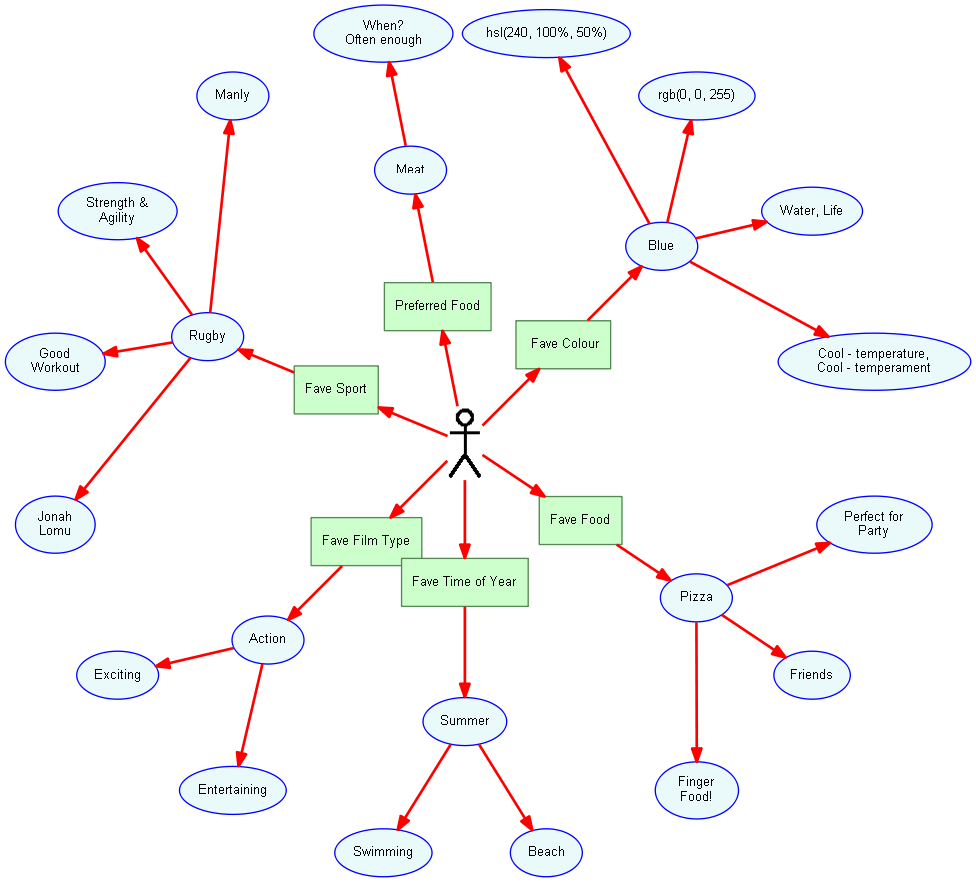
\includegraphics[scale=0.5]{concept-map.png}
\vspace*{1.5 cm}

\newpage
\bibliographystyle{apa}
\bibliography{biblist}

\end{document}
